\section{Models}
Here the basic definitions, the general models concept, and a list of
models available in \Dumux are given. The actual differential equations
can be found in the localresiduals (see doxygen documentation of the
model's \texttt{LocalResidual} class).

\subsection{Basic Definitions and Assumptions}
The basic definitions and assumptions are made, using the example
of a three-phase three-component system water-NAPL-gas
\cite{A3:class:2002a}. The modification for other multicomponent
systems is straightforward and can be found, e.\ g., in
\cite{A3:bielinski:2006,A3:acosta:2006}.

\begin{description}
\item[Components:]
The term \emph{component} stands for constituents of the phases which
can be associated with a unique chemical species, or, more generally, with
a group of species exploiting similar physical behavior. In this work, we
assume a water-gas-NAPL system composed of the phases water (subscript
$\text{w}$), gas ($\text{g}$), and NAPL ($\text{n}$). These phases are
composed of the components water (superscript $\text{w}$), the pseudo-component
air ($\text{a}$), and the organic contaminant ($\text{c}$) (see Fig.
\ref{fig:phaseMassEnergyTransfer}).

\item[Phases:]
For compositional multi-phase models, \emph{phases}
are not only matter of a single chemical substance. Instead, their
composition in general includes several species/components. For mass transfer,
the component behavior is quite different from the phase behavior.

\item[Equilibrium:]
For the non-isothermal, multi-phase, multi-component processes in porous media
we state that the assumption of \emph{local thermodynamic equilibrium}.
Chemical equilibrium means that the mass/mole fractions of a component in
different phases are in equilibrium.
Thermal equilibrium assumes the same temperature for all considered phases.
Mechanical equilibrium is not valid in a porous medium, since discontinuities
in pressure can occur across a fluid-fluid interface due to capillary effects.

\item[Notation:]
The subscript index $\alpha \in \{\text{w}, \text{n}, \text{g}\}$ refers
to the phase, while the superscript $\kappa \in \{\text{w}, \text{a}, \text{c}\}$
refers to the component.
\end{description}

\begin{table}
\begin{tabular}{llll}
$p_\alpha$ & phase pressure & $\phi$ & porosity \\
$T$ & temperature & $K$ & absolute permeability tensor \\
$S_\alpha$ & phase saturation & $\tau$ & tortuosity \\
$x_\alpha^\kappa$ & mole fraction of component $\kappa$ in phase $\alpha$ & $\boldsymbol{g}$ & gravitational acceleration \\
$X_\alpha^\kappa$ & mass fraction of component $\kappa$ in phase $\alpha$ & $q^\kappa_\alpha$ & volume source term of $\kappa$ in $\alpha$ \\
$\varrho_{\text{mol},\alpha}$ & molar density of phase $\alpha$ & $u_\alpha$ & specific internal energy \\
$\varrho_{\alpha}$ & mass density of phase $\alpha$ & $h_\alpha$ & specific enthalpy \\
$M$ & molar mass of a phase or component & $c_\text{s}$ & specific heat enthalpy \\
$k_{\text{r}\alpha}$ & relative permeability & $\lambda_\text{pm}$ & heat conductivity \\
$\mu_\alpha$ & phase viscosity & $q^h$ & heat source term \\
$D_\alpha^\kappa$ & diffusivity of component $\kappa$ in phase $\alpha$ & $\boldsymbol{v}_{a,\alpha}$  & advective velocity \\
$\boldsymbol{v}_\alpha$ & velocity (Darcy or free flow)& & \\
\end{tabular}
\caption{Notation list for most of the variables and indices used in \Dumux.}

\end{table}

\begin{figure}
  \centering
  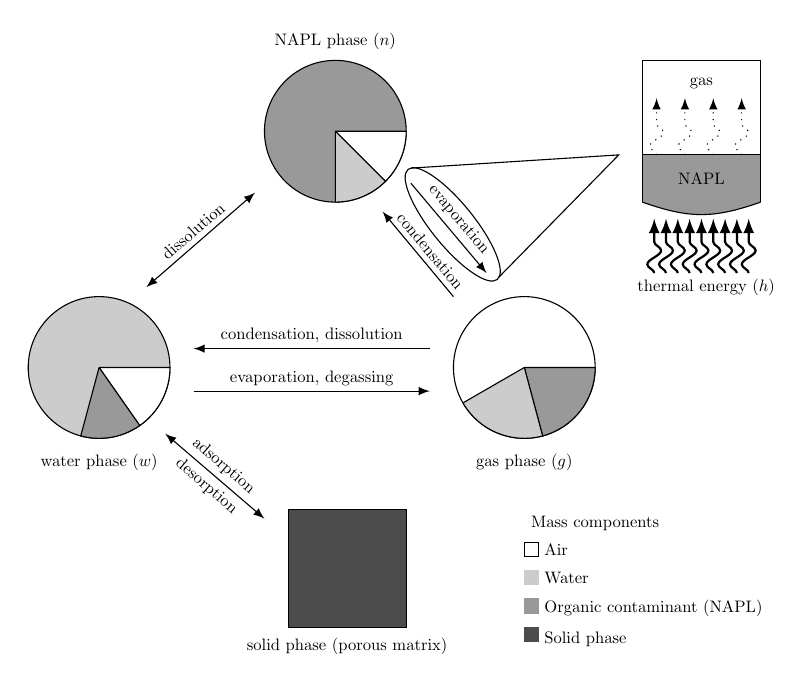
\begin{tikzpicture} [>=latex,scale=0.6, every node/.style={transform shape}]
    % Ellipse 1 solid
    \coordinate (A) at (1,-0.5);
    \draw [fill=black!70](A) rectangle(3.5,2) node at(2.25,-0.9) {solid phase (porous matrix)};
    % Ellipse 2 water
    \coordinate (B) at (-3,5);
    \draw [fill=black!20](B) circle(1.5cm);
    \node [yshift=5mm]at(-3,2.5){water phase $(w)$};
    \draw[fill=white] (B)--+(1.5,0)arc(0:-55:1.5cm)--(B);
    \draw[fill=black!40] (B)--+(-55:1.5cm)arc(-55:-105:1.5cm)--(B);
    % Ellipse 3 gas
    \coordinate (C) at (6,5);
    \draw [](C) circle (1.5cm);
    \node[yshift=5mm]at(6,2.5){gas phase $(g)$};
    \draw [fill=black!40](C)--+(1.5,0)arc(0:-75:1.5cm)--(C);
    \draw [fill=black!20] (C)--+(-75:1.5cm)arc(-75:-150:1.5cm)--(C);
    % Ellipse 4 napl
    \coordinate (D) at (2,10);
    \draw [fill=black!40](D) circle (1.5cm);
    \node[yshift=5mm]at(2,11.4){NAPL phase $(n)$};
    \draw [fill=white](D)--+(1.5,0)arc(0:-45:1.5cm)--(D);
    \draw [fill=black!20] (D)--+(0,-1.5)arc(-90:-45:1.5cm)--(D);
    % arrows
    %A-B
      \draw [<->,white](0.5,1.8)--(-1.6,3.6) node[black,above,sloped,pos=0.5]{adsorption};
      \draw [<->](0.5,1.8)--(-1.6,3.6) node[below,sloped,pos=0.5]{desorption};
    %B-C
      \draw[<-](-1,5.4)--(4,5.4)node[above,sloped,pos=0.5]{condensation, dissolution};
      \draw[->](-1,4.5)--(4,4.5)node[above,sloped,pos=0.5]{evaporation, degassing};
    %B-D
      \draw[<->](-2,6.7)--(0.3,8.7)node[above,sloped,pos=0.5]{dissolution};
    %D-C
      \draw[->](3.6,8.9)--(5.2,7)node[above,sloped,pos=0.5]{evaporation};
      \draw[rotate around={-51:(4,6.8)}](3.35,7.95) ellipse (1.5cm and 0.45cm);  %Ellipse um evaporation
      \draw (3.6,9.22)--(8,9.5)--(5.45,6.9);
      \draw[<-](3,8.3)--(4.5,6.5)node[above,sloped,pos=0.55]{condensation};
    % thermal energy
    \filldraw [black!40](8.5,9.5)rectangle(11,8.5);
    \draw (8.5,9.5)rectangle(11,11.5);
    \draw (8.5,9.5)--(8.5,8.5);
    \draw (11,9.5)--(11,8.5);
    \draw [decorate,decoration={bent,aspect=0.4,amplitude=6},fill=black!40](11,8.5)--(8.5,8.5);
    \foreach \x in {8.75,9,...,10.8}
    \draw [->,decorate,decoration={snake,post length=2mm},thick](\x,7)--(\x,8.15);
    \foreach \x in {8.8,9.4,10,10.6}
    \draw [->,dotted,decorate,decoration={snake,post length=2mm}](\x,9.5)--(\x,10.7);
    \node at(9.75,11){gas};
    \node at(9.75,9){NAPL};
    \node at(9.85,6.7){thermal energy $(h)$};
    % legende
    \node at (7.5,1.7){Mass components};
    \draw[](6,1)rectangle +(0.3,0.3) node at(6.3,1.15) [right]{Air};
    \filldraw[black!20](6,0.4) rectangle +(0.3,0.3) node at (6.3,0.55)[black,right]{Water};
    \filldraw[black!40](6,-0.2) rectangle +(0.3,0.3) node at (6.3,-0.1)[right,black]{Organic contaminant (NAPL)};
    \filldraw[black!70](6,-0.8) rectangle +(0.3,0.3) node at (6.3,-0.75)[right,black]{Solid phase};
  \end{tikzpicture}
  \caption{Mass and energy transfer between the phases}
  \label{fig:phaseMassEnergyTransfer}
\end{figure}


\subsection{Gas mixing laws}
Prediction of the $p-\varrho-T$ behavior of gas mixtures is typically based on two (contradicting) concepts: Dalton's law or Amagat's law.
In the following the two concepts will be explained in more detail.
%
\subsubsection{Dalton's law}
Dalton's law assumes that the gases in the mixture are non-interacting (with each other) and each gas independently applies its own pressure (partial pressure), the sum of which is the total pressure:
%
\begin{equation}
p = \sum_{i}^{}p_i.
\end{equation}
Here $p_i$ refers to the partial pressure of component i.
As an example, if two equal volumes of gas A and gas B are mixed, the volume of the mixture stays the same but the pressures add up (see Figure \ref{fig:dalton1}).
%
\begin{figure}[ht]
	\centering
	\includegraphics[width=0.7\textwidth]{PNG/dalton1.png}
	\caption{Dalton's law visualized}
	\label{fig:dalton1}
\end{figure}
%
The density of the mixture, $\varrho$, can be calculated as follows:
\begin{equation}
\varrho = \frac{m}{V} = \frac{m_\mathrm{A} + m_\mathrm{B}}{V} = \frac{\varrho_\mathrm{A} V + \varrho_\mathrm{B} V}{V} = \varrho_\mathrm{A} + \varrho_\mathrm{B},
\end{equation}
%
or for an arbitrary number of gases:
\begin{equation}
\varrho = \sum_{i}^{} \varrho_i ; \quad \varrho_m = \sum_{i}^{} \varrho_{m,i}.
\end{equation}
%
\subsubsection{Amagat's law}
Amagat's law assumes that the volumes of the component gases are additive; the interactions of the different gases are the same as the average interactions of the components. This is known as Amagat's law:
%
\begin{equation}
V = \sum_{i}^{}V_i.
\end{equation}
%
As an example, if two volumes of gas A and B at equal pressure are mixed, the pressure of the mixture stays the same, but the volumes add up (see Figure \ref{fig:dalton2}).
%
\begin{figure}[ht]
	\centering
	\includegraphics[width=0.7\textwidth]{PNG/dalton2.png}
	\caption{Amagat's law visualized}
	\label{fig:dalton2}
\end{figure}
%
The density of the mixture, $\varrho$, can be calculated as follows:
\begin{equation}
\varrho = \frac{m}{V} = \frac{m}{V_\mathrm{A} + V_\mathrm{B}} = \frac{m}{\frac{m_\mathrm{A}}{\varrho_\mathrm{A}} \frac{m_\mathrm{B}}{\varrho_\mathrm{B}}} =
\frac{m}{\frac{X_\mathrm{A} m}{\varrho_\mathrm{A}} \frac{X_\mathrm{B} m}{\varrho_\mathrm{B}}} = \frac{1}{\frac{X_\mathrm{A}}{\varrho_\mathrm{A}} \frac{X_\mathrm{B}}{\varrho_\mathrm{B}}},
\end{equation}
%
or for an arbitrary number of gases:
%
\begin{equation}
\varrho = \frac{1}{\sum_{i}^{}\frac{X_i}{\varrho_i}}  ; \quad  \varrho_m = \frac{1}{\sum_{i}^{}\frac{x_i}{\varrho_{m,i}}}.
\end{equation}
%
\subsubsection{Ideal gases}
An ideal gas is defined as a gas whose molecules are spaced so far apart that the behavior of a molecule is not influenced by the presence of other molecules.
This assumption is usually valid at low pressures and high temperatures. The ideal gas law states that, for one gas:
%
\begin{equation}
p = \varrho \frac{RT}{M} ; \quad p= \varrho_m RT.
\end{equation}
%
Using the assumption of ideal gases and either Dalton's law or Amagat's law lead to the density of the mixture, $\varrho$, as:
%
\begin{equation}
\varrho = \frac{p}{RT} \sum_{i}^{}M_i x_i ; \quad \varrho_m = \frac{p}{RT}.
\end{equation}
%
\subsection{Available Models}
A list of all available models can be found
in the Doxygen documentation at
\url{http://www.dumux.org/doxygen-stable/html-\DumuxVersion/modules.php}.
The documentation includes a detailed description for every model.

\subsubsection{Time discretization}

Our systems of partial differential equations are discretized in space and in time.

Let us consider the general case of a balance equation of the following form
\begin{equation}\label{eq:generalbalance}
\frac{\partial m(u)}{\partial t} + \nabla\cdot\mathbf{f}(u, \nabla u) + q(u) = 0,
\end{equation}
seeking an unknown quantity $u$ in terms of storage $m$, flux $\mathbf{f}$ and source $q$.
All available Dumux models can be written mathematically in form of \eqref{eq:generalbalance}
with possibly vector-valued quantities $u$, $m$, $q$ and a tensor-valued flux $\mathbf{f}$.
For the sake of simplicity, we assume scalar quantities $u$, $m$, $q$ and a vector-valued
flux $\mathbf{f}$ in the notation below.

For discretizing \eqref{eq:generalbalance} we need to choose an
approximation for the temporal derivative $\partial m(u)/\partial t$.
While many elaborate methods for this approximation exist,
we focus on the simplest one of a first order difference quotient
\begin{equation}\label{eq:euler}
\frac{\partial m(u_{k/k+1})}{\partial t}
\approx \frac{m(u_{k+1}) - m(u_k)}{\Delta t_{k+1}}
\end{equation}
for approximating the solution $u$ at time $t_k$ (forward) or $t_{k+1}$ (backward).
The question of whether to choose the forward or the backward quotient leads to the
explicit and implicit Euler method, respectively.
In case of the former, inserting \eqref{eq:euler} in \eqref{eq:generalbalance}
at time $t_k$ leads to
\begin{equation}\label{eq:expliciteuler}
\frac{m(u_{k+1}) - m(u_k)}{\Delta t_{k+1}} + \nabla\cdot\mathbf{f}(u_k, \nabla u_k) + q(u_k) = 0,
\end{equation}
whereas the implicit Euler method is described as
\begin{equation}\label{eq:impliciteuler}
\frac{m(u_{k+1}) - m(u_k)}{\Delta t_{k+1}}
+ \nabla\cdot\mathbf{f}(u_{k+1}, \nabla u_{k+1}) + q(u_{k+1}) = 0.
\end{equation}
Once the solution $u_k$ at time $t_k$ is known, it is straightforward
to determine $m(u_{k+1})$ from \eqref{eq:expliciteuler},
while attempting to do the same based on \eqref{eq:impliciteuler}
involves the solution of a nonlinear system.
On the other hand, the explicit method \eqref{eq:expliciteuler} is stable only
if the time step size $\Delta t_{k+1}$ is below a certain limit that depends
on the specific balance equation, whereas the implicit method \eqref{eq:impliciteuler}
is unconditionally stable.

\subsubsection{Algorithms to solve equations}
The governing equations of each model can be solved monolithically or sequentially.
The basic idea of the sequential algorithm is to reformulate the
equations of multi-phase flow into one equation for
pressure and equations for phase/component/... transport. The pressure equation
is the sum of the mass balance equations and thus considers the total flow of the
fluid system. The new set of equations is considered as decoupled (or weakly coupled)
and can thus be solved sequentially. The most popular sequential model is the
fractional flow formulation for two-phase flow which is usually implemented applying
an IMplicit Pressure Explicit Saturation algorithm (IMPES).
In comparison to solving the equations monolothically, the sequential structure allows the use of
different discretization methods for the different equations. The standard method
used in the sequential algorithm is a cell-centered finite volume method. Further schemes,
so far only available for the two-phase pressure equation, are cell-centered finite
volumes with multi-point flux approximation (MPFA O-method) and mimetic finite differences.
An $h$-adaptive implementation of both sequential algorithms is provided for two dimensions.
